\chapter{LPWAN}
Il principale problema che si presenta nella ottica del IoT è avere una
infrastruttura di rete capace di gestire il traffico di milioni di dispositivi
contemporaneamente connessi. Fino ad oggi la principale tecnologia wireless
usata nelle comunicazioni M2M \emph{Machine to Machine} è stata la rete
cellulare.   La scelta della rete 2G, 3G, 4G è svantaggiosa nel ambito del IoT
poiché offre data-rate molto maggiore rispetto a quello normalmente utilizzato
dalle applicazioni M2M, comportando l'uso di moduli radio sovradimensionati e
andando ad aumentare di molto il prezzo per unità.  Inoltre, l'elevato consumo
energetico e il prezzo svantaggioso degli abbonamenti offerti dagli operatori
telefonici, ha portato alla ricerca di nuove soluzioni basate su frequenze ISM o
licenziate.  In questo capitolo verranno elencate le principali tecnologie
presenti nel mercato, mettendone in evidenza le differenze che le
contraddistinguono.

\section{LPWAN}
Per colmare il gap tra tecnologie esistenti e la necessita di connettere milioni
di devices diversi, sono nate le  LPWAN \emph{Low power wide area network}.
Con questo termine, si identificano tutte quelle reti ideate appositamente per
l'IoT, le quali garantiscono una ampio raggio di azione, andando a sacrificare
il bit rate e la complessità dei moduli radio.

\begin{figure}[h]
    \centering 
        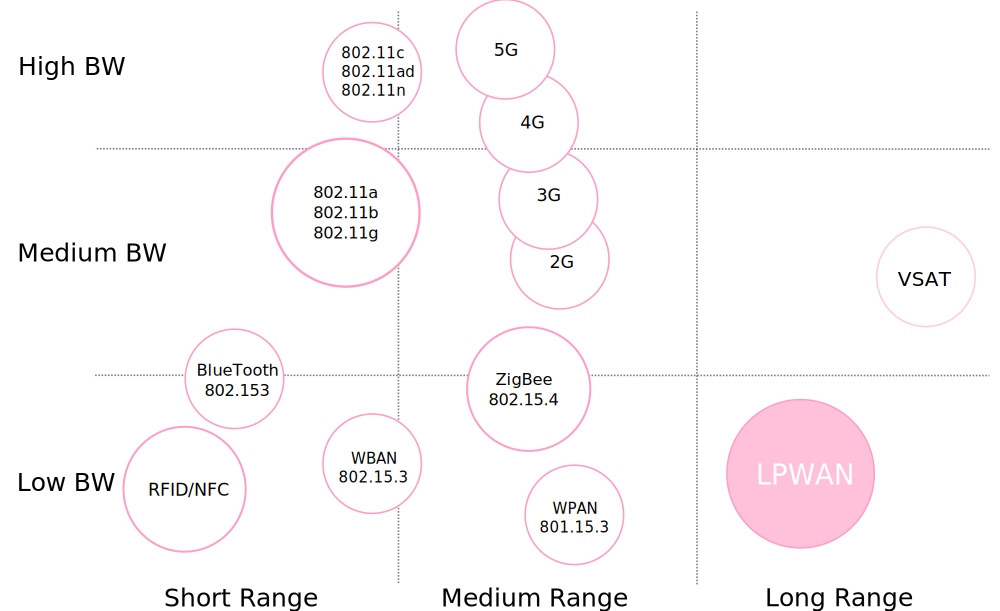
\includegraphics[width=16cm]{network-com}
    \caption{Comparazione tipologia di reti}
\end{figure}

In questo contesto, i maggiori competitor sono Lora, Sigfox, NB-IoT, EC-GSM-IoT
e LTE-M.  Anche se ognuna di queste reti punta a ottenere la leadership del
mercato, esse implementano soluzioni tecniche molto diverse tra di loro, ognuna
delle quali ha vantaggi e svantaggi a seconda del contesto nel quale viene
utilizzata.


\section{NB-IoT}
Narrowband IoT (NB-IoT) o LTE Cat NB1 è uno standard certificato nella release 13 del 3GPP, la
quale riutilizza le infrastrutture già presenti, quali 2G, 3G, 4G per la rapida
realizzazione di una rete LPWA per l'IoT.
Focalizzandosi sulla durata della batteria, i moduli NB-IoT risultano avere un
costo all'unità minore del 75\% rispetto ad un normale modulo LTE.
Basato frequenze licenziate, NB-IoT è in grado di
offrire tre diversi scenari di sviluppo \cite{NB-white_paper}
\begin{itemize}
\item \emph{standalone}, utilizzando qualsiasi spettro disponibile del
operatore.
\item \emph{guard band}, utilizzando lo spettro libero presente tra due bande
radio, per prevenire interferenze.
\item \emph{in band}, utilizzando lo stesso spettro della banda LTE.
\end{itemize}
\begin{figure}[h]
    \centering 
        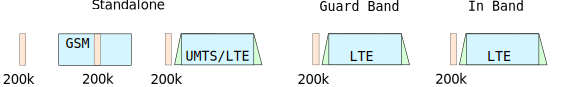
\includegraphics[width=16cm]{nb-iot}
    \caption{Modalità di funzionamento NB-IoT}
\end{figure}
L'obbiettivo che NB-IoT si prefigge è quello di mettere a disposizione una
tecnologia con una elevata copertura ed un basso data-rate. La possibilità di
riutilizzare strutture già esistenti, ed il basso costo per device , rendo
NB-IoT, una delle tecnologie che sta riscuotendo maggiore successo nel abito IoT.



\section{LTE-M}
Dalla realise 8 del 3GPP, diverse nuove tipologie di rete LTE sono disponibili.
La categoria che offre le migliori performance batteria/data-rate è la categoria
LTE Cat-M1 o LTE-M.
LTE-M a differenza del NB-IoT, rispecchia LTE in pieno, quindi implementa due
moduli di ricezione, è full duplex supportando la Frequency Division Multiplexing
(FDM) e Time Division Multiplexing (TDM). Risultando adatto per applicazioni con
esigenze diverse da quelle del NB-IoT, è in grado di raggiunger i 5Mbps in
uplink e 10[Mbps] in downlink teorici.  Questo tipo di connessione sarà utile
per tutte quelle applicazioni in cui è richiesta una elevata sicurezza del dato
da trasmettere, come ad esempio applicazioni di video-sorveglianza o automotive
.Questa tecnologia ,già disponibile negli Stati Uniti tramite la rete Verizon, è
in fase di roll out per molti operatori europei.

\section{EC-GSM-IoT}
EC-GSM-IoT si basa su funzionalità aggiuntive a partire da EGPRS che consentono
ad una rete GSM/EDGE di essere predisposta per fornire servizi IoT. Lo standard
è stato pensato in particolare per quei Paesi, come quelli in via di sviluppo,
dove una rete LTE non è ancora disponibile. L’occupazione spettrale di ogni
canale corrisponde a  200 kHz.  Tuttavia, al fine di dispiegare EC-GSM-IoT, si
richiede una banda utile di 2.4 MHz per permettere il frequency hopping , che,
con l’aggiunta di 2 canali di guardia di 200 kHz ciascuno agli estremi della
banda, porta l’occupazione di banda complessiva a 2.8 MHz.  La
potenza di trasmissione del Il data rate di picco raggiungibile sia in DL sia in
UL è di 491 kbps, mentre il valore mediato nominale è di 98 kbps sia in DL sia
in UL. Al fine di soddisfare i requisiti di capacità (più di 50.000 terminali in
ogni singolo settore di una cella trisettoriale). 

La figura \ref{tab:IoT_cell_comp} riassume in breve le varie caratteristiche
delle reti cellulari facenti parte della categoria LPWA
\begin{table}[h]
    \centering 
                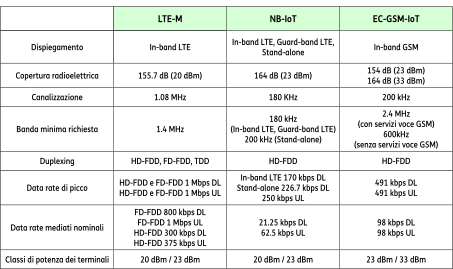
\includegraphics[width=16cm]{tim_iot}
    \caption{Comparazione reti cellulari per l'IoT}
    \label{tab:IoT_cell_comp} 
\end{table}



\section{Sigfox}
SigFox, azienda francese, sta sviluppando in partnership con altri operatori di
rete una soluzione LPWAN basata sulla sua tecnologia. Sigfox punta alla
costruzione di una rete mondiale proprietaria basata su frequenze ISM.
Correntemente SigFox è presente in Francia, Belgio, Olanda e Portogallo come
illustrato nella figura \ref{fig:Sig_covereg}.
\begin{figure}[h]
    \centering 
                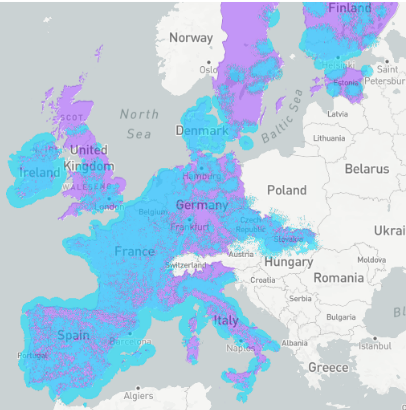
\includegraphics[width=11cm]{SigFox_covereg}
    \caption{Mappa copertura SigFox}
    \label{fig:Sig_covereg} 
\end{figure}

Gli end-devices comunicano con le varie base stations usando una modulazione (BPSK)
\emph{Binary Phase Shift Keying} con una banda di soli 100[Hz]. 
Per via delle regolazioni vigenti nello spettro ISM, è per garantire una durata
della batteria pari ad una decina di anni, il numero massimo di messaggi
inviabili in un giorno è 140, con lunghezza del payload pari a 12[byte] e un
throughput pari a 100[bps]. SigFox si colloca come rete LPWAN con il minore
throughput, limitando il numero di use-case possibili. Inizialmente SigFox
supportava solo comunicazioni unidirezionali, successivamente, ha introdotto la
possibilità di avere una comunicazione bidirezionale, limitando il numero di
byte trasmissibili da gateway a devices a 4-8 bytes per giorno.

\section{LoRaWAN}
\emph{LoraWAN} è una tecnologia di modulazione wireless semi-proprietaria 
sviluppata da Semtech. Essa è composta da un layer fisico ,proprietario, che
prende il nome di \emph{Lora}\cite{LoRaCss101} , e una parte libera chiamata 
LoRaWAN\cite{LoRaWAN101} nella quale viene definito un protocollo di comunicazione, 
il quale usa LoRa come layer fisico. 
Basandosi su una tecnica di comunicazione a \emph{spread spectrum}, LoRa è in
grado di instaurare una comunicazione bidirezionale tra device e gateway.
I punti chiave dei questa tecnologia, sono il grande raggio di copertura , il 
basso consumo energetico e la capacità di adattare in maniera dinamica il
data rate, il quale può variare dai 0.3 ai 50[Kbps] a seconda dell'utilizzo. 
Come per SigFox, la tecnologia sviluppata da Semtech, si basa sulle bande ISM,
inoltre Essendo il protocollo LoRaWAN open source, si ha la possibilità di
creare delle reti pubbliche o private senza disporre di alcuna licenza, 
riducendo così il time to market di questa tecnologia.  
Progetti come \href{https://www.thethingsnetwork.org/}{The Things Network}
mirano a creare una rete LoRa ,pubblica è privata,  a livello globale.
\section{Osservazioni}
In questo mercato frammentato, non è semplice capire quale tecnologia sia adatta
a ricoprire una data applicazione. Essendo questi standard molto giovani, è
difficile comprendere le reali potenzialità di ognuna di queste soluzioni.
Quello che è possibile prevedere, sarà un incremento esponenziale di device che
stanno alla base della piramide in figura \ref{fig:pyramid}, devices i quali
potranno essere utilizzati in innumerevoli settori, non ancora esplorati dalle
tecnologie attuali, come per esempio i contatori della dell'acqua, applicazioni
per l'agricoltura di precisione ecc. 

\begin{figure}[h]
    \centering 
                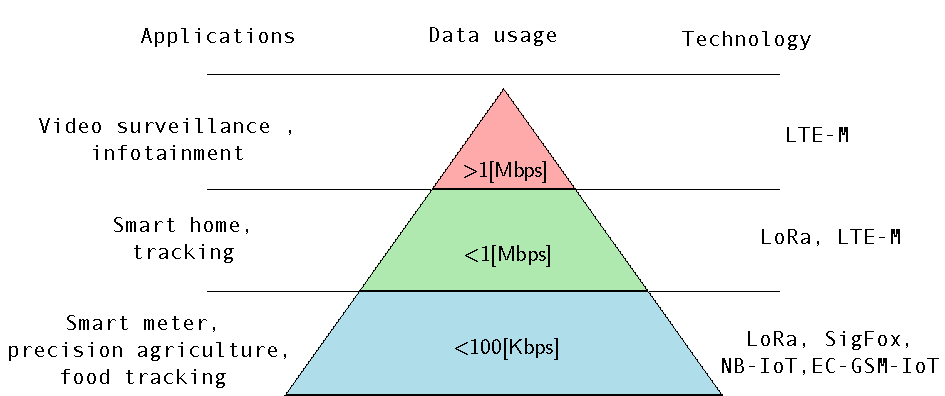
\includegraphics[width=11cm]{pyramid}
    \caption{Capacità delle reti LPWA}
    \label{fig:pyramid} 
\end{figure}

\pagebreak
Per le aziende, che si apprestano ad investire sul mondo dell'IoT, la scelta
della corretta tecnologia su cui andare a sviluppare i loro servizi non risulta
semplice, in quanto, fattori quali sicurezza, aggiornamenti software,
affidabilità devono essere ancora testate a pieno. Con la figura
\ref{fig:feature_comp} si vuole riassumere in breve i punti chiave delle
tecnologie appena trattate.

\begin{figure}[h]
    \centering 
                \includegraphics[width=11cm]{Comparsion_no_line}
    \caption{Comparazione feature reti LPWAN}
    \label{fig:feature_comp} 
\end{figure}

Nel prossimo capitolo verrà analizzata in dettaglio la soluzione che Semtech
propone, approfondendo il layer fisico \emph{Lora} e la struttura del protocollo
LoRaWAN.
